\documentclass[11pt,a4paper]{article}

\usepackage[T1]{fontenc}
\usepackage[utf8]{inputenc}
\usepackage[french]{babel}
\usepackage{lmodern}
\usepackage{geometry}
\usepackage{microtype}
\usepackage{xcolor}
\usepackage{hyperref}
\usepackage{booktabs}
\usepackage{enumitem}
\usepackage{listings}
\usepackage{fancyhdr}
\usepackage{graphicx}
\usepackage{float}

\geometry{margin=2.35cm}
\setlength{\headheight}{14pt}
\hypersetup{colorlinks=true,linkcolor=blue!55!black,urlcolor=blue!55!black,pdftitle={TeachToLearn -- Rapport Hackathon SCIA 2026},pdfauthor={Clovis Lefebvre et Evariste Balvay}}
\setlist{noitemsep,topsep=4pt}
\pagestyle{fancy}
\fancyhf{}
\lhead{TeachToLearn}
\rhead{Hackathon SCIA 2026}
\cfoot{\thepage}
\lstset{basicstyle=\ttfamily\small,breaklines=true,frame=single,rulecolor=\color{black!25},backgroundcolor=\color{black!03},columns=fullflexible}

\title{\textbf{TeachToLearn}\\[0.35em]\large Une salle de classe 3D multi-agents pour apprendre en enseignant}
\author{Clovis Lefebvre \and Evariste Balvay}
\date{Hackathon SCIA 2026 --- Septembre 2026}

\begin{document}
\maketitle

\begin{abstract}
Ce rapport présente \textit{TeachToLearn}, notre réponse au sujet «~IA agentique au service de l'éducation~» du Hackathon SCIA 2026. Le projet transforme une salle de classe 3D en exercice de pédagogie active~: l'utilisateur prépare un cours, l'enseigne à une classe composée de plusieurs agents IA, puis reçoit une évaluation argumentée. L'originalité de la proposition repose moins sur un simple chatbot que sur l'orchestration de personnages autonomes, aux rôles pédagogiques complémentaires, qui disposent de contextes séparés et décident individuellement d'intervenir ou de rester silencieux.
\end{abstract}

\tableofcontents
\newpage

\section{Contexte et intention}

Le support du Hackathon SCIA 2026 proposait deux sujets sur une durée annoncée de 48 heures. Nous avons choisi le premier~: concevoir une IA agentique capable d'apprendre, de planifier et d'agir afin d'améliorer concrètement une situation d'apprentissage. Le critère mis en avant par le jury était l'innovation, et non l'optimisation d'un benchmark.

Notre point de départ est la méthode de Feynman~: expliquer une notion à quelqu'un constitue un test exigeant de compréhension. Or, apprendre seul face à un cours statique ne met pas suffisamment l'apprenant en situation de reformuler, de répondre aux objections ou de s'adapter à des niveaux de compréhension différents. \textit{TeachToLearn} place donc l'utilisateur dans le rôle d'un professeur remplaçant. Il doit préparer puis donner un cours court devant une classe simulée, dont les membres réagissent selon leurs personnalités.

L'ambition n'était pas de construire un environnement scolaire réaliste dans tous ses détails. Nous avons cherché à rendre crédible le mécanisme pédagogique essentiel~: passer de la préparation théorique à l'explication, à la confrontation avec des questions, puis à un retour structuré.

\section{Expérience utilisateur et déroulé du jeu}

L'application est une salle de classe low-poly en 3D, navigable à la première personne. Les déplacements utilisent \texttt{ZQSD}, la caméra est contrôlée à la souris et un réticule permet de sélectionner les personnages. Le chat est volontairement intégré à cette scène plutôt qu'isolé dans une interface de messagerie classique~: l'utilisateur donne un cours \emph{dans} une classe, face à des interlocuteurs incarnés.

Le scénario est organisé en trois étapes.

\subsection{Étape 1 --- Briefing avec l'examinateur}

La partie commence avec M.~Vautier, l'examinateur pédagogique. L'utilisateur indique le sujet à traiter. L'agent propose alors entre trois et cinq notions essentielles, puis répond aux questions de préparation. Pendant cette phase, la conversation est verrouillée~: l'utilisateur ne peut pas ouvrir un autre chat, fermer le briefing ou parler à la classe. Ce choix évite de casser le scénario avant que les objectifs ne soient définis.

\begin{figure}[H]
  \centering
  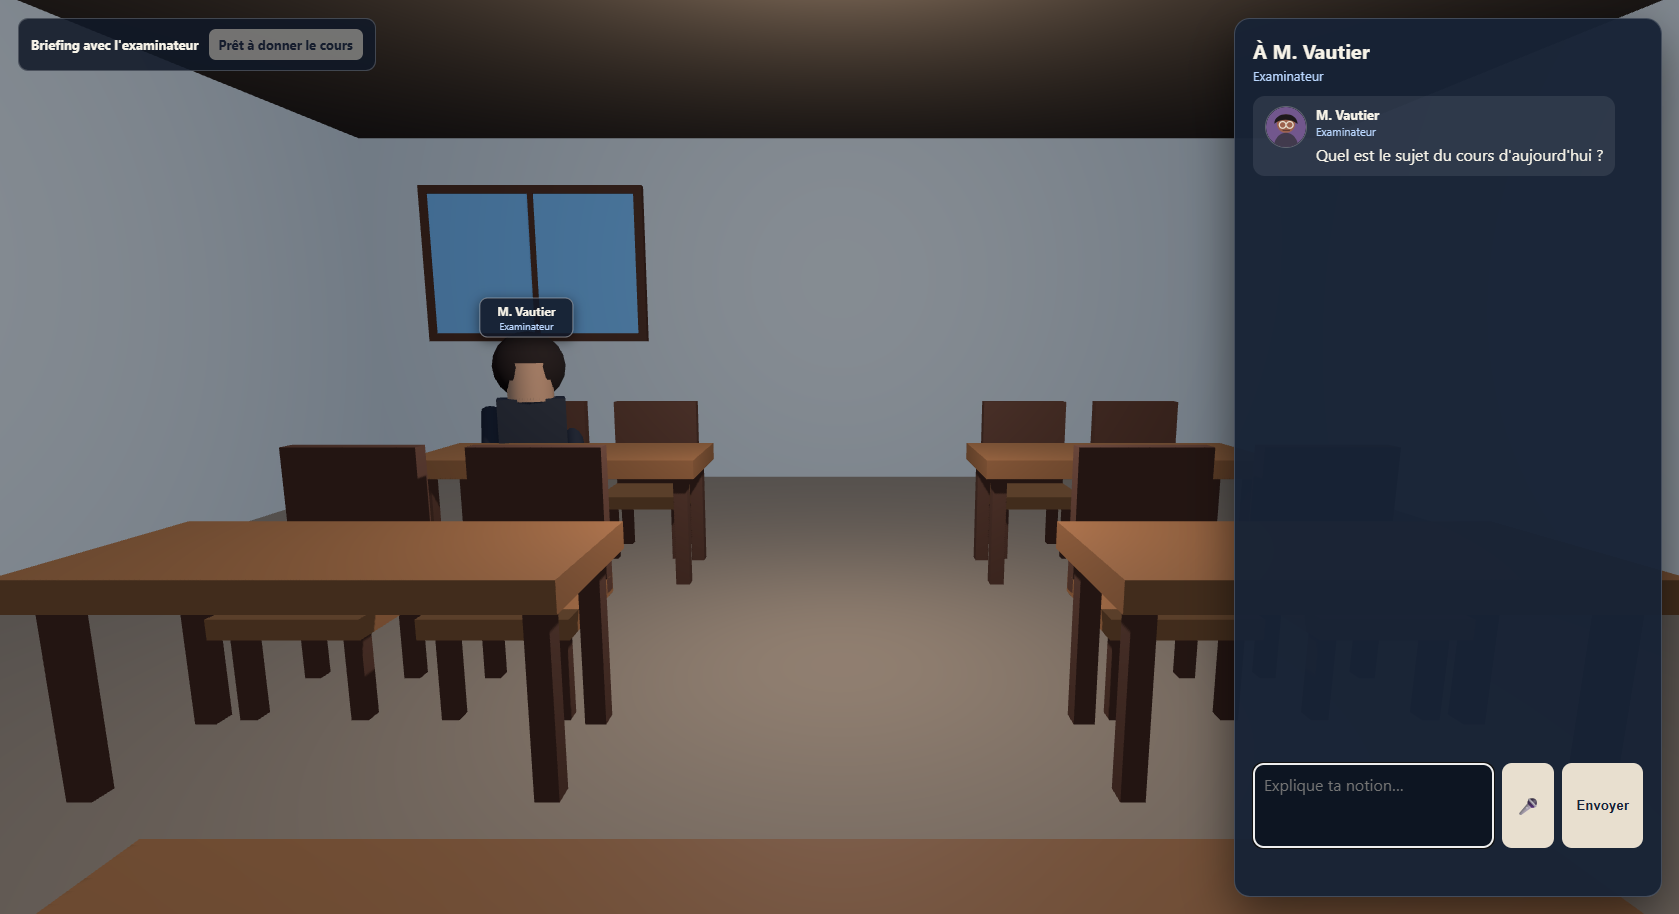
\includegraphics[width=0.92\textwidth]{rapport-images/01-briefing-m-vautier.png}
  \caption{Entretien de briefing avec M.~Vautier~: l'examinateur demande à l'utilisateur de préciser le sujet du cours.}
  \label{fig:briefing-vautier}
\end{figure}

Les objectifs sont transmis par le modèle sous une métadonnée structurée~:

\begin{lstlisting}
[[OBJECTIVES:["notion 1", "notion 2"]]]
\end{lstlisting}

Cette ligne est retirée du texte visible du chat puis convertie en une liste d'objectifs affichée à gauche de l'écran.

\begin{figure}[H]
  \centering
  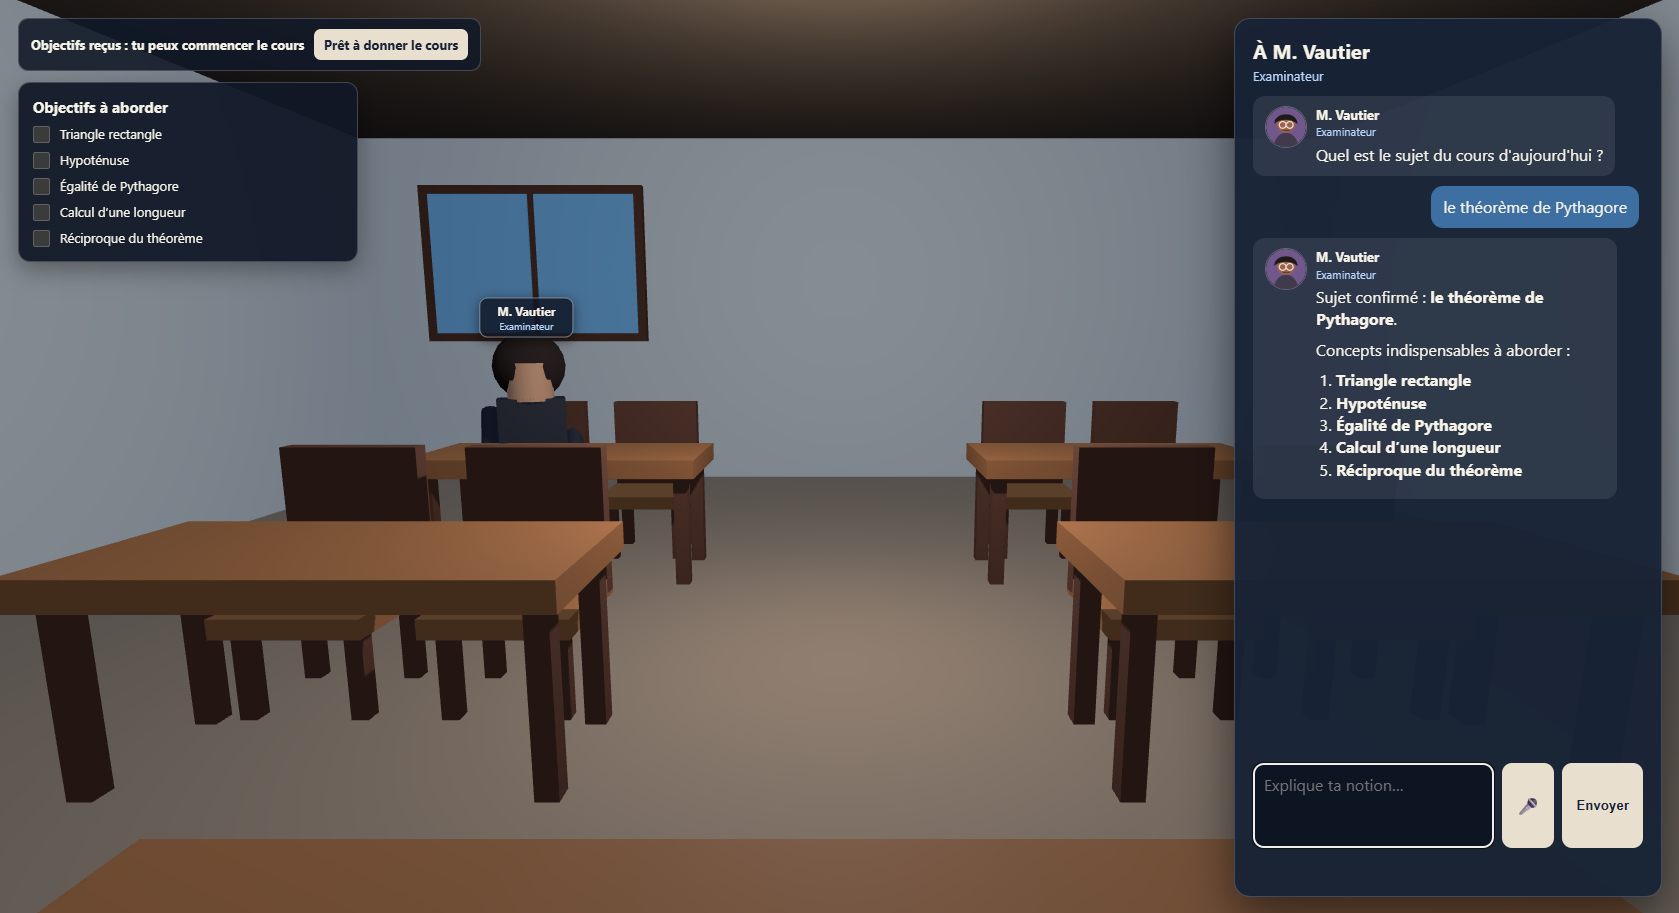
\includegraphics[width=0.92\textwidth]{rapport-images/02-objectifs-convenus.png}
  \caption{Objectifs convenus avec M.~Vautier pour le cours sur le théorème de Pythagore, affichés dans le panneau persistant à gauche.}
  \label{fig:objectifs-convenus}
\end{figure}

\subsection{Transition vers l'étape 2}

Lorsque l'utilisateur choisit «~Prêt à donner le cours~», une transition par fondu noir masque le changement de phase. Les élèves apparaissent pendant cet écran, puis le chat de classe s'ouvre. Au-delà de l'effet visuel, cette transition marque le passage de l'apprenant préparé au professeur qui doit maintenant mettre ses connaissances en pratique.

\subsection{Étape 2 --- Enseignement face à la classe}

L'utilisateur explique les notions dans le chat général. Il peut taper son message ou utiliser la reconnaissance vocale du navigateur pour dicter du texte en français. Un bouton microphone est affiché seulement si l'API Web Speech est disponible. La transcription est insérée dans le champ de saisie, sans envoi automatique, afin de permettre une relecture avant de parler à la classe.

Les objectifs définis par M.~Vautier restent visibles. Ils ne sont pas déclarés validés pendant le cours~: seules des cases à cocher neutres sont affichées. Ce sont les preuves présentes dans la transcription du professeur qui décideront de leur validation finale.

\begin{figure}[H]
  \centering
  \includegraphics[width=\textwidth]{rapport-images/04-enseignement-classe.png}
  \caption{Étape 2~: l'utilisateur enseigne face à la classe et échange avec les élèves dans le chat général.}
\end{figure}

\subsection{Étape 3 --- Évaluation finale}

Le cours s'achève soit par le bouton «~Terminer le cours~», soit lorsque M.~Vautier juge nécessaire d'interrompre la séance avec le marqueur \texttt{[END\_COURSE]}. Le formulaire, le champ de saisie, le bouton d'envoi et les conversations avec les personnages sont alors verrouillés. Le bilan reste à l'écran et seul le bouton «~Relancer une partie~» permet de recommencer.

L'évaluation produit une note sur 20, des points forts, des axes de progrès et un verdict pour chaque objectif. Le modèle fournit ce verdict dans une seconde métadonnée structurée~:

\begin{lstlisting}
[[OBJECTIVE_RESULTS:[true, false, true]]]
\end{lstlisting}

Le client transforme ces booléens en cases cochées ou décochées dans le panneau d'objectifs.

\begin{figure}[H]
  \centering
  \includegraphics[width=\textwidth]{rapport-images/05-evaluation-finale-m-vautier.png}
  \caption{Étape 3~: bilan final de M.~Vautier, avec la note, les points forts et les axes de progrès.}
\end{figure}

\section{Le coeur du projet~: une classe multi-agents}

\subsection{Pourquoi plusieurs agents~?}

Une seule IA capable de jouer tous les élèves aurait été plus simple à implémenter, mais moins intéressante pédagogiquement. Un tel agent tend à homogénéiser les réactions, à changer de rôle au sein d'une même réponse et à produire un dialogue artificiel. Notre architecture sépare au contraire les points de vue. Chaque personnage reçoit une identité, une consigne et une mémoire qui lui sont propres.

\begin{table}[h]
\centering
\begin{tabular}{p{3cm}p{4cm}p{7cm}}
\toprule
\textbf{Agent} & \textbf{Rôle} & \textbf{Apport pédagogique} \\
\midrule
Alex & L'intello & Vérifie la rigueur, relève les erreurs factuelles et pose des questions techniques courtes. \\
Lucas & Le perturbateur & Interroge l'utilité concrète d'une notion et pousse le professeur à donner des exemples accessibles. \\
Sam & L'élève perdu & Demande des reformulations, confond les bases et met à l'épreuve la clarté de l'explication. \\
M.~Vautier & L'examinateur & Surveille la cohérence du cours, recadre les dérives importantes et conduit le briefing comme l'évaluation. \\
\bottomrule
\end{tabular}
\caption{Répartition des rôles dans la classe multi-agents.}
\end{table}

\subsection{Orchestration d'un tour de parole}

Quand le professeur envoie un message à la classe, le client lance quatre requêtes \texttt{classroom} en parallèle, une pour Alex, Lucas, Sam et M.~Vautier. Pour chacun, il construit un contexte constitué de~:

\begin{itemize}
  \item sa mémoire de conversation privée avec le professeur~;
  \item la transcription commune de la classe~;
  \item la liste des objectifs à enseigner~;
  \item son prompt de personnalité et de rôle pédagogique.
\end{itemize}

Chaque agent décide s'il a une contribution utile. S'il n'en a pas, il renvoie le marqueur \texttt{[SILENCE]}, qui n'est pas affiché au joueur et n'est pas réinjecté comme une intervention de classe. Sinon, sa réponse apparaît avec son portrait et est ajoutée à la mémoire collective. Cette décision distribuée permet d'éviter que tous les personnages répondent mécaniquement à chaque phrase.

Le choix d'appels parallèles réduit également le temps d'attente perçu~: les quatre agents réfléchissent au même moment. En contrepartie, ils ne se répondent pas dans le même tour~; ils découvrent les prises de parole retenues au tour suivant via la transcription commune. C'est un compromis assumé entre réactivité, simplicité et cohérence conversationnelle.

\section{Architecture technique}

\subsection{Pile logicielle}

\begin{itemize}
  \item \textbf{TypeScript} pour la logique applicative~;
  \item \textbf{Three.js} pour la scène 3D, le rendu WebGL, les interactions par raycasting et les labels CSS2D~;
  \item \textbf{Vite} pour le développement, le build et un middleware serveur \texttt{/api/chat}~;
  \item \textbf{OpenAI Chat Completions} en streaming pour les agents~;
  \item \textbf{KaTeX} pour rendre le Markdown mathématique et les formules LaTeX dans le chat~;
  \item \textbf{Web Speech API} pour la dictée vocale gratuite lorsque le navigateur la prend en charge.
\end{itemize}

Le projet reste volontairement léger~: il ne dépend pas d'un framework front-end lourd. Le DOM du chat est manipulé directement et la scène 3D est assemblée à partir de modules dédiés aux objets, aux déplacements, aux collisions et au gameplay.

\subsection{Organisation du code}

\begin{lstlisting}
main.ts                 Scene Three.js et raccordement des modules
scene/                  Salle, materiaux et eclairage
objects/                Bureau, chaises, tableau, porte, fenetre et personnages
player/                 Controles, collisions, interactions et phases du jeu
chat/conversation.ts    Chat, memoires, Markdown, LaTeX et orchestration agents
vite.config.ts          Endpoint /api/chat, prompts et streaming OpenAI
player/objectives.ts    Panneau d'objectifs et cases de validation
\end{lstlisting}

La clé OpenAI reste côté serveur, chargée à partir du fichier \texttt{.env}. Le navigateur n'y accède jamais directement. Le middleware valide les modes de conversation, le nombre de messages, leur taille, ainsi que la forme de la liste d'objectifs avant de contacter l'API externe.

\section{Rendu des réponses et interfaces de communication}

Le chat ne se limite pas au texte brut. Les réponses agents sont interprétées comme du Markdown~: titres, listes, emphase, liens, citations et blocs de code sont rendus dans le DOM. Les expressions mathématiques LaTeX sont rendues avec KaTeX~; les formats \verb|$...$|, \verb|\(...\)|, \verb|$$...$$| et \verb|\[...\]| sont pris en charge. En cas de formule invalide, le texte initial reste visible plutôt que de casser l'affichage.

Le rendu évite l'injection de HTML brut généré par le modèle~: les éléments sont construits avec des nœuds DOM et \texttt{textContent}. KaTeX est utilisé avec l'option \texttt{trust: false}. Cette décision est importante puisque le contenu affiché provient d'une IA distante.

\section{Une évaluation fondée sur des preuves}

Une difficulté apparue pendant les itérations concernait la note finale~: un utilisateur pouvait entrer dans la classe, ne rien dire et recevoir malgré tout une bonne évaluation. La cause était double~: le briefing pouvait être confondu avec un cours, et le modèle pouvait considérer les paroles des élèves comme des preuves de maîtrise.

Nous avons corrigé ce point à deux niveaux.

\begin{enumerate}
  \item \textbf{Garde déterministe côté client~:} si aucun message de rôle \texttt{user} n'a été envoyé à la classe, l'application n'appelle pas le modèle d'évaluation. Elle affiche directement une note de 0/20 et marque tous les objectifs comme non validés.
  \item \textbf{Prompt d'évaluation strict~:} la transcription envoyée à l'évaluation ne contient que l'étape 2. Le système demande explicitement de n'évaluer que les messages du professeur. Une notion n'est validée que si elle est expliquée de manière explicite, correcte et suffisamment claire. Une mention isolée, une question, le briefing ou une réponse d'élève ne constituent pas une preuve.
\end{enumerate}

Cette correction illustre une leçon importante du projet~: dans une application éducative, les composants déterministes doivent encadrer les décisions d'un modèle génératif lorsqu'elles ont un impact sur l'évaluation de l'utilisateur.

\section{Itérations et difficultés rencontrées}

Le développement a été guidé par des problèmes observés lors de la mise en situation.

\begin{itemize}
  \item \textbf{Cohérence du scénario~:} le briefing pouvait initialement être quitté ou remplacé trop tôt. Il a été verrouillé jusqu'à la transition vers la classe.
  \item \textbf{Lisibilité des objectifs~:} les notions annoncées oralement par l'examinateur étaient difficiles à retenir. Elles sont devenues une interface persistante avec une validation finale par cases à cocher.
  \item \textbf{Passage entre les étapes~:} le changement brutal de salle rendait le scénario moins lisible. Un fondu noir a été ajouté afin de signaler la bascule vers le cours.
  \item \textbf{Fin de partie~:} après le bilan, il ne doit plus être possible de recommencer une conversation avec un personnage. Le chat est donc verrouillé et un bouton de relance réinitialise la partie.
  \item \textbf{Silence des agents~:} la présence de \texttt{[SILENCE]} devait rester une décision ponctuelle, non une instruction persistante. Les silences sont filtrés avant l'affichage et la mémorisation collective.
  \item \textbf{Accessibilité de saisie~:} la dictée vocale a été ajoutée sans imposer de dépendance payante ni envoyer de fichier audio au serveur applicatif.
\end{itemize}

\section{Limites et perspectives}

Le prototype a des limites assumées. Les objectifs sont générés à partir d'un sujet donné dans le chat~: l'ingestion d'un PDF et un système de récupération de connaissances ne sont pas encore implémentés. Les historiques sont conservés en mémoire dans le navigateur et disparaissent au rechargement. Le middleware \texttt{/api/chat} est fourni par Vite en développement~; un déploiement robuste nécessiterait un véritable service backend. Enfin, la qualité des interactions dépend du modèle configuré, de la connexion et du respect des contraintes de prompt.

Les évolutions naturelles seraient~:

\begin{itemize}
  \item importer un cours ou un PDF pour extraire des objectifs sourcés~;
  \item persister les sessions, les résultats et les progrès de l'utilisateur~;
  \item ajouter une orchestration séquentielle ou un agent coordinateur pour permettre des échanges plus riches entre élèves~;
  \item enrichir les critères de validation avec des rubriques explicitables et un suivi longitudinal~;
  \item proposer une solution de reconnaissance vocale locale pour les navigateurs non compatibles avec la Web Speech API.
\end{itemize}

\section{Conclusion}

\textit{TeachToLearn} propose une lecture concrète de l'IA agentique appliquée à l'éducation~: non pas un assistant unique qui donne la réponse, mais une situation d'apprentissage dans laquelle plusieurs agents incarnent les contraintes d'une vraie classe. Alex demande de la précision, Lucas force la contextualisation, Sam vérifie la simplicité et M.~Vautier structure le parcours puis évalue les preuves d'enseignement.

En 48 heures de hackathon, nous avons privilégié une expérience complète~: briefing, objectifs, passage en scène, interactions multi-agents, évaluation fiable, rendu mathématique et dictée vocale. Le projet reste un prototype, mais il démontre qu'une architecture multi-agents peut transformer un chat en outil de mise en pratique pédagogique.

\vfill
\begin{center}
\textit{Rapport signé par Clovis Lefebvre \& Evariste Balvay}
\end{center}

\end{document}